% !TeX program = lualatex -synctex=1 -interaction=nonstopmode --shell-escape %.tex

\documentclass[_international_finance_p1.tex]{subfiles}
\beamertemplatenavigationsymbolsempty


%\newcommand{\onslidecell}[2]{\onslide<#1->{#2}}
\newcommand{\aheader}[2]{\action<#1-|alert@#1>{#2}}
\begin{document}
\section{Binomial Options Pricing Model (BOPM)}
\subsection{Market Volatility}
\setbeamercovered{transparent}
\begin{frame}{Binomial Options Pricing Model (BOPM)}
\begin{itemize}[<+->]
\item
Buyer and seller always have different opinions on the underlying instrument price direction
\item
At each step, it is assumed that the underlying instrument will move up or down by a specific factor ($u$ or $d$) per step of the tree (where, by definition, $u \ge 1$ and $0 < d \le 1 )$.
\item
The up and down factors are calculated using the underlying volatility, $\sigma$, and the time duration of a step, $t$, measured in time intervals (days, months, years).
\item
Binomial Options Pricing Model says nothing about the underlying instrument up or down price movements probability.
\end{itemize}
\end{frame}
\begin{frame}{}
\begin{itemize}[<+->]
\item
At each final node of the tree — i.e. at expiration of the option — the option value is simply its intrinsic, or exercise, value.

    $Max [ (S_n-K), 0 ]$, for a call option
    
    $Max [ (K – S_n), 0 ]$, for a put option:

Where $K$ is the strike price and $S_n$ is the spot price of the underlying asset at the $n^{th}$ period. 
\item
The binomial pricing model traces the evolution of the option`s key underlying variables in discrete-time. This is done by means of a binomial lattice (tree), for a number of time steps between the valuation and expiration dates. Each node in the lattice represents a possible price of the underlying at a given point in time.
\end{itemize}
\end{frame}
\setbeamercovered{invisible}
\begin{frame}[shrink=15]{USDRUB quotes changes from 01.10.2013 to 01.10.2014}
\begin{center}
% Table generated by Excel2LaTeX from sheet 'USDRUB'
\begin{table}[htbp]
  \centering
    \begin{tabular}{>{\onslide<1->}c
    				>{\onslide<1->}c        
    				>{\onslide<2->}c}
    \toprule
    \multicolumn{1}{c}{Date} & \multicolumn{1}{c}{Close price} & \multicolumn{1}{c}{$\Delta,\%$} \\
    \midrule
    01.10.2013 & 32,0973 &  \\
    01.11.2013 & 33,0852 & 3,08\% \\
    01.12.2013 & 32,8311 & -0,77\% \\
    01.01.2014 & 35,2523 & 7,37\% \\
    01.02.2014 & 35,9238 & 1,90\% \\
    01.03.2014 & 35,1707 & -2,10\% \\
    01.04.2014 & 35,6287 & 1,30\% \\
    01.05.2014 & 34,8855 & -2,09\% \\
    01.06.2014 & 33,9675 & -2,63\% \\
    01.07.2014 & 35,705 & 5,12\% \\
    01.08.2014 & 37,1041 & 3,92\% \\
    01.09.2014 & 39,5562 & 6,61\% \\
    01.10.2014 & 42,9913 & 8,68\% \\
    \bottomrule
    \end{tabular}%
  \label{tab:addlabel}%
\end{table}%
\end{center}
\end{frame}
\begin{frame}{Monthly USDRUB quotes graph}
\begin{center}
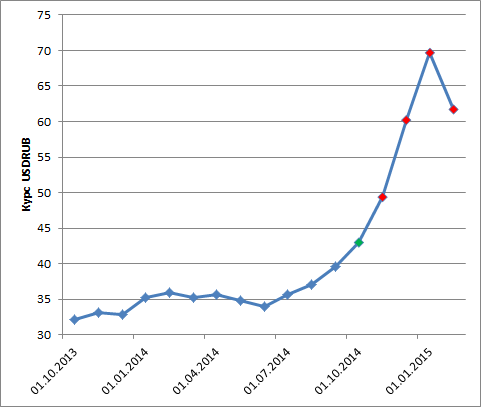
\includegraphics[scale=0.7]{img/usdrubquoteschart}
\end{center}
\end{frame}
\begin{frame}{Monthly USDRUB quote percentage change}
\begin{center}
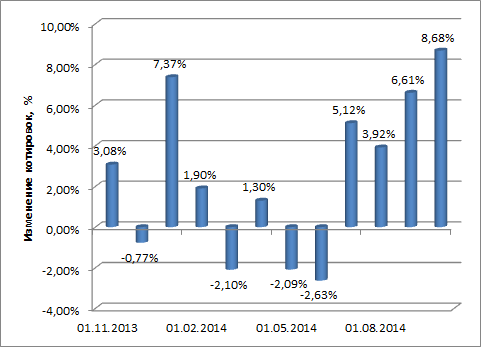
\includegraphics[scale=0.8]{img/usdrubdeltaperc}
\end{center}
\end{frame}
\begin{frame}{USDRUB quotes percentage change intervals}
\begin{center}
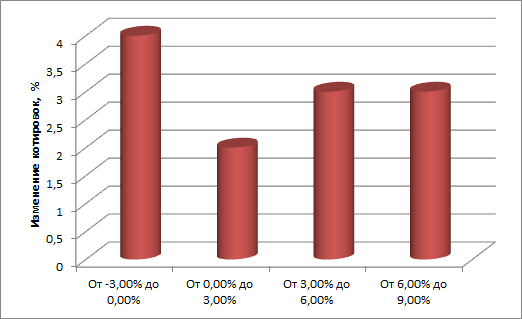
\includegraphics[scale=0.8]{img/usdrubquotesintervals}
\end{center}
\end{frame}
\setbeamercovered{transparent}
\begin{frame}{Formulas for the average return and the standard deviation of return}
\begin{itemize}[<+->]
\item
The average return:
$$m=\frac{\sum_{i=1}^n x_i}{n}$$
where $x_i$ – observed value;

$n$ – number of values.
\item
The standard deviation of return:
$$s=\sqrt{\frac{\sum_{i=1}^n (m-x_i)^2}{n-1}}$$
\end{itemize}
\end{frame}
\setbeamercovered{invisible}
\begin{frame}[shrink=15]{Monthly USDRUB average return and its standard deviation}
% Table generated by Excel2LaTeX from sheet 'Расчет m и s'
\begin{table}[htbp]
  \centering
    \begin{tabular}{cccc}
    \toprule
    & $x_i$    & $m-x_i$  & $(m-x_i)^2$ \\
    \midrule
1 & 3,08\% & \hiddencell{4}{-0,54\%} & \hiddencell{5}{0,30} \\
2 & -0,77\% & \hiddencell{4}{3,30\%} & \hiddencell{5}{10,90} \\
3 & 7,37\% & \hiddencell{4}{-4,84\%} & \hiddencell{5}{23,44} \\
4 & 1,90\% & \hiddencell{4}{0,63\%} & \hiddencell{5}{0,40} \\
5 & -2,10\% & \hiddencell{4}{4,63\%} & \hiddencell{5}{21,44} \\
6 & 1,30\% & \hiddencell{4}{1,23\%} & \hiddencell{5}{1,52} \\
7 & -2,09\% & \hiddencell{4}{4,62\%} & \hiddencell{5}{21,34} \\
8 & -2,63\% & \hiddencell{4}{5,17\%} & \hiddencell{5}{26,68} \\
9 & 5,12\% & \hiddencell{4}{-2,58\%} & \hiddencell{5}{6,66} \\
10 & 3,92\% & \hiddencell{4}{-1,38\%} & \hiddencell{5}{1,92} \\
11 & 6,61\% & \hiddencell{4}{-4,08\%} & \hiddencell{5}{16,61} \\
12 & 8,68\% & \hiddencell{4}{-6,15\%} & \hiddencell{5}{37,83} \\
    \midrule
    $\Sigma$& \hiddencell{2}{30,40\%} 
    &  - 
    & \onslide<6->{169,02} \\
    \textbf{m}
    & \hiddencell{3}{\textit{\textbf{2,5337\%}}} 
    & \textbf{s}
    & \hiddencell{7}{\textit{\textbf{3,9199\%}}} \\
    \bottomrule
    \end{tabular}%
  \label{tab:addlabel}%
\end{table}%

\end{frame}
\begin{frame}{Monthly USDRUB average return and its standard deviation}
\begin{center}

% Table generated by Excel2LaTeX from sheet 'Расчет m и s'
\begin{table}[htbp]
  \centering
    \begin{tabular}{lr}
    \toprule
    m     & 2,5337\% \\
    s     & 3,9199\% \\
    \midrule
    m+s   & 6,4535\% \\
    m-s   & -1,3862\% \\
    \midrule
    u     & 1,0645 \\
    d     & 0,9861 \\
    \bottomrule
    \end{tabular}%
  \label{tab:addlabel}%
\end{table}%
\end{center}
\end{frame}
\subsection{Binomial price tree}
\begin{frame}{Create the binomial price tree}
{Options call and put parameters}
\begin{center}
% Table generated by Excel2LaTeX from sheet 'Модель'
\begin{table}[htbp]
  \centering
    \begin{tabular}{lrr}
    \toprule
    & \multicolumn{2}{c}{Option type} \\  \cmidrule{2-3}
    & Call & Put \\
    \midrule
    Option price & 45,00 ~₽ & 45,00 ~₽ \\
    Term & 2 month & 2 month \\
    USD rate, \% annual & 1\% & 1\% \\
    RUB rate, \% annual & 8,00\% & 8,00\% \\
    USD rate, \% monthly & 0,08\% & 0,08\% \\
    RUB rate, \% monthly & 0,67\% & 0,67\% \\
    \bottomrule
    \end{tabular}%
  \label{tab:addlabel}%
\end{table}%
\end{center}
\end{frame}


\setbeamercovered{invisible}
\begin{frame}[fragile,shrink=35]{The binomial price tree}
\begin{center}

\end{center}
\end{frame}
\newcommand{\optionpicturescale}{1.2}
\begin{frame}[fragile,shrink=35]{The binomial price tree}
\begin{figure}
	\center
	\begin{overprint}
		\forloop{slideno}{1}{\value{slideno} < 7}{%
			\only<\value{slideno}>{
				\includegraphics[page=\value{slideno},
				scale=\optionpicturescale
				% trim={<left> <lower> <right> <upper>}				
				,trim={0cm 2cm 0cm 0cm}
				,clip]
				{tikz/price_binary_tree}}}
	\end{overprint}
	\caption{The binomial price tree}
\end{figure}

\end{frame}
\subsection{Intermediate Option Value}
\setbeamercovered{transparent}
\begin{frame}{}
\begin{itemize}[<+->]
\item
The option value for each earlier node is found, starting at the penultimate time step, and working back to the first node of the tree (the valuation date) where the calculated result is the value of the option.
\item
The "arbitrage free" approach creates a position that has an identical value in either state – the cash flow in one period is therefore known, and arbitrage pricing is applicable. 
\end{itemize}
\end{frame}
\begin{frame}{}
\begin{itemize}[<+->]
\item
In case of an option the equivalent position consists of some amount of the base and quoted currency (one long and the other short) which has the value identical to the option price at the each moment.
\item
Under the risk neutrality assumption, today's fair price of a derivative is equal to the expected value of its future payoff discounted by the risk free rate. Therefore, expected value is calculated using the option values from the later two nodes.
\end{itemize}
\end{frame}


\begin{frame}{}
\begin{itemize}[<+->]
\item
The expected value is then discounted at r, the risk free rate corresponding to the life of the option. 
\item
Long position in one currency yields interest revenue
\item
Short position in the other currency cause interest cost
\item
Usually the interest revenue/expenses are calculated on the basis of the risk free rate (e.g. LIBOR).
\end{itemize}
\end{frame}
\setbeamercovered{invisible}
\begin{frame}[shrink=10]{Option value at earlier nodes calculation example}
\begin{align*}
\begin{cases} 
\onslide<2->{z_1 = 45,7658 \cdot x_1 + y_1}\\ 
\onslide<3->{3,7193 = 48,7193 \cdot x_1 \cdot (1 + \frac{r_{USD}}{n}) + y_1 \cdot (1 + \frac{r_{RUB}}{n})}\\
\onslide<4->{0,1314 = 45,1314 \cdot x_1 \cdot (1 + \frac{r_{USD}}{n}) + y_1 (1 + \cdot \frac{r_{RUB}}{n})}
\end{cases}
\end{align*}
$z_1$ – the option value at each intermediate node;

$x_1$ – base currency position amount, negative value means short position;

$y_1$ – quoted currency position amount, negative value means short position;

$r_{USD},r_{RUB}$ – risk free deposit/lending rate, in the base and quoted currency respectively, annual

$n$ - interest rate compounding frequency (number of compounding periods per year, e.g. 12 months).
\end{frame}
\setbeamercovered{transparent}
\begin{frame}{}
\begin{itemize}[<+->]
\item
Call and put options pricing is the same. The difference is only in options pricing at the final periods.
\item
If exercise is permitted at the node, then the model takes the greater of binomial and exercise value at the node.
\end{itemize}
\end{frame}
\setbeamercovered{invisible}
\subsection{Call and Put Options}
\begin{frame}[fragile,shrink=35]{Call option}
\begin{figure}
	\center
	\begin{overprint}
		\forloop{slideno}{1}{\value{slideno} < 6}{%
			\only<\value{slideno}>{
				\includegraphics[page=\value{slideno},
				scale=\optionpicturescale
				% trim={<left> <lower> <right> <upper>}				
				,trim={0cm 2cm 0cm 0cm}
				,clip]
				{tikz/option_call}}}
	\end{overprint}
	\caption{Option call}
\end{figure}
\end{frame}
\begin{frame}[fragile,shrink=35]{Put option}
\begin{figure}
	\center
	\begin{overprint}
		\forloop{slideno}{1}{\value{slideno} < 8}{%
			\only<\value{slideno}>{
				\includegraphics[page=\value{slideno},
				scale=\optionpicturescale
				% trim={<left> <lower> <right> <upper>}				
				,trim={0cm 2cm 0cm 0cm}
				,clip]
				{tikz/option_put}}}
	\end{overprint}
	\caption{Option put}
\end{figure}
\end{frame}
\subsection{Binary options}
\begin{frame}{Binary options pricing}
{Binary options parameters}
\begin{center}

% Table generated by Excel2LaTeX from sheet 'Модель'
\begin{table}[htbp]
  \centering
    \begin{tabular}{lrr}
    \toprule
    & \multicolumn{2}{c}{Option type} \\  \cmidrule{2-3}
    & One touch & No touch \\
    \midrule
    Barrier price & 48,00 ~₽ & 42,50 ~₽ \\
    Payoff & \$1 000 & \$1 000 \\
    Term & 2 months & 2 months \\
    USD rate, \% annual & 1\% & 1\% \\
    RUB rate, \% annual & 8,00\% & 8,00\% \\
    USD rate, \% monthly & 0,08\% & 0,08\% \\
    RUB rate, \% monthly & 0,67\% & 0,67\% \\
    \bottomrule
    \end{tabular}%
  \label{tab:addlabel}%
\end{table}%
\end{center}
\end{frame}
\begin{frame}[fragile,shrink=35]{One touch option}
\begin{figure}
	\center
	\begin{overprint}
		\forloop{slideno}{1}{\value{slideno} < 9}{%
			\only<\value{slideno}>{
				\includegraphics[page=\value{slideno},
				scale=\optionpicturescale
				% trim={<left> <lower> <right> <upper>}				
				,trim={0cm 2cm 0cm 0cm}
				,clip]
				{tikz/option_one_touch}}}
	\end{overprint}
	\caption{One touch option}
\end{figure}
\end{frame}
\begin{frame}[fragile,shrink=35]{No touch option}
\begin{figure}
	\center
	\begin{overprint}
		\forloop{slideno}{1}{\value{slideno} < 9}{%
			\only<\value{slideno}>{
				\includegraphics[page=\value{slideno},
				scale=\optionpicturescale
				% trim={<left> <lower> <right> <upper>}				
				,trim={0cm 2cm 0cm 0cm}
				,clip]
				{tikz/option_no_touch}}}
	\end{overprint}
	\caption{No touch option}
\end{figure}
\end{frame}
\setbeamercovered{transparent}
\subsection{General one period model}
\begin{frame}[shrink=15]{General one period model}
\begin{figure}
	\center
	\begin{overprint}
		\forloop{slideno}{1}{\value{slideno} < 2}{%
			\only<\value{slideno}>{
				\includegraphics[page=\value{slideno},
				scale=\optionpicturescale
				% trim={<left> <lower> <right> <upper>}				
				,trim={0cm 7cm 0cm 0cm}
				,clip]
				{tikz/option_general_model}}}
	\end{overprint}
	\caption{General one period model}
\end{figure}

where

$S$ - undelying asset current price;

$E$ - options execution price.
\begin{align}
C_u = \begin{cases} u \cdot S - E, & \mbox{for } u \cdot S > E \\ 
0, & \mbox{for } u \cdot S \leq E \end{cases}\\
C_d = \begin{cases} d \cdot S - E, & \mbox{for } d \cdot S > E \\ 
0, & \mbox{for } d \cdot S \leq E \end{cases}
\end{align}
\end{frame}
\begin{frame}[shrink=15]{System of equations for one period model}{and its solution}
\begin{align}
\begin{cases} 
C = S \cdot x + y\\ 
C_u = u \cdot S \cdot x \cdot r_{USD} + y \cdot r_{RUB}\\
C_d = d \cdot S \cdot x \cdot r_{USD} + y \cdot r_{RUB}
\end{cases}\\[12pt]
x=\frac{C_u-C_d}{(u-d)\cdot S \cdot r_{USD}}
y=\frac{u \cdot C_d-d \cdot C_u}{(u-d) \cdot r_{RUB}}
\end{align}
\begin{align}
C = S \cdot x + y
\end{align}

where

$x, y$ - position amounts in dollars and rouble, respectively;

$r_{USD},r_{RUB}$ - deposit/lending rates for time period \textit{T} in dollars and roubles, respectively.
\end{frame}


\end{document}